\subsection{Validación cruzada}
La validación cruzada o cross-validation es una técnica utilizada para evaluar los resultados de un análisis estadístico cuando el conjunto de datos se ha segmentado en una muestra de entrenamiento y otra de prueba, la validación cruzada comprueba si los resultados del análisis son independientes de la partición. Aunque la validación cruzada es una técnica diseñada para modelos de regresión y predicción, su uso se ha extendido a muchos otros ejercicios de machine learning.
https://bookdown.org/content/2274/metodos-de-clasificacion.html#validacion-cruzada

\begin{figure}[H]
 \centering	
   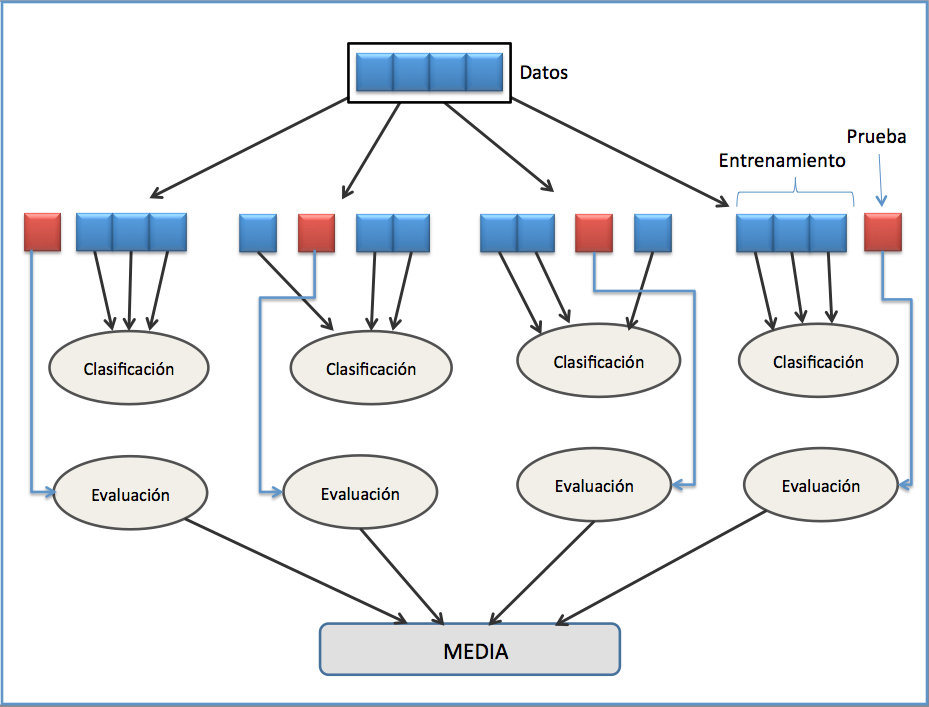
\includegraphics[width=0.4\textwidth]{images/Esquema.png}
   \caption{\textit{Cromatografía interrelaciona la parte física, química y biológica del suelo.}}
   \end{figure}	


